\documentclass[12pt,a4paper,titlepage]{scrartcl}

\usepackage{comment}
\usepackage[main=ngerman,english]{babel}
\usepackage[utf8]{inputenc}
\usepackage[T1]{fontenc}
\usepackage{lmodern}
\usepackage{geometry}
\geometry{left=2.5cm,right=2.5cm,top=2.5cm,bottom=3cm,head=29pt,foot=25pt}
\setlength{\footheight}{25pt}
\usepackage{microtype}
\usepackage{amsmath,amssymb,mathtools}
\numberwithin{equation}{section}
\numberwithin{table}{section}
\numberwithin{figure}{section}
\usepackage{siunitx}
\sisetup{locale=US, separate-uncertainty=true, per-mode=fraction}
\usepackage{booktabs}
\usepackage{multirow}
\usepackage{graphicx}
\usepackage{float}
\usepackage{caption}
\usepackage{subcaption}
\usepackage[automark]{scrlayer-scrpage}
\usepackage[most]{tcolorbox}
\usepackage{hyperref}
\usepackage{pdfpages}
\usepackage{csvsimple-l3}
\usepackage{longtable}
\usepackage{graphicx}


\input{../../jupyterpackages.tex}

% jupyter nbconvert --to latex 'Path'
% enferne usepackages und begin{document} und end{document}
% \input in main.tex mit \input{Path}


\newcommand{\pdfabbildung}[2]{%
    \refstepcounter{figure}%
    \addcontentsline{lof}{figure}{\protect\numberline{\thefigure}#1}%
    \label{#2}%
}

\newcommand{\pdftabelle}[2]{%
    \refstepcounter{table}%
    \addcontentsline{lot}{table}{\protect\numberline{\thetable}#1}%
    \label{#2}%
}


\hypersetup{colorlinks=true, linkcolor=blue!60!black, urlcolor=blue!60!black, citecolor=blue!60!black}

\clearpairofpagestyles

\chead{%
    \versuch\hfill\autor\\
    \rule{\textwidth}{0.2pt}%
}
\cfoot{%
    \rule{\textwidth}{0.2pt}\\[-0.5ex]
    \pagemark\ 
}
\addtokomafont{pagefoot}{\small}
\setlength{\parindent}{0pt}

\newtcolorbox{resultbox}[1][]{ 
    enhanced,
    colback=black!4!white,
    colframe=black!65!black,
    boxrule=0.8pt,
    arc=0.0mm,
    title=#1,
    fonttitle=\bfseries,
    %drop shadow
}


\newcommand{\versuch}{Versuch 34}
\newcommand{\titel}{Spektralphotometrie}
\newcommand{\praktikum}{Physikalisches Anfängerpraktikum 1}
\newcommand{\autor}{Jonathan Gießen}
\newcommand{\gruppe}{Gruppe 8}
\newcommand{\datum}{14. September 2026}
\newcommand{\betreuer}{Lucija Ruzic}

\begin{document}

\pagestyle{scrheadings}

\begin{titlepage}



    \centering
    \vspace*{4cm}
    {\large Universität Heidelberg\par}
    {\small Fakultät für Physik und Astronomie\par}
    {\Large \praktikum\par}
    \vspace{0.8cm}
    {\LARGE \bfseries \versuch\ -- \titel\par}
    \vspace{1.5cm}

    \begin{tabular}{ll}
        \textbf{Autor:} & \autor\\
        \textbf{Gruppe:} & \gruppe\\
        \textbf{Betreuer:} & \betreuer\\
        \textbf{Versuchsdatum:} & \datum\\
    \end{tabular}

    \vfill
    \hrulefill\
\end{titlepage}

\tableofcontents

\bigskip
\begin{tcolorbox}[colback=gray!5,colframe=gray!60,boxrule=0.8pt,arc=0.01mm,title=KI-Hinweis]
    Für die sprachliche Formulierung dieses Protokolls wurde in Teilen in Einleitung \ref{sec:Einleitung} Textgenerierung verwendet. 
\end{tcolorbox}
\clearpage


\section{Einleitung}\label{sec:Einleitung}
In diesem Versuch 34 wird die Fotometrie eingeführt, unter anderem, um die Konzentrationsbestimmung einer Substanz durch die Absorption von Licht zu untersuchen. Das primäre Ziel des Versuches ist es, das Absorptionsspektrum einer Lösung mit der Lebensmittelfarbe Brillantblau FCF aufzunehmen und den molaren Extinktionskoeffizienten zu bestimmen. Die Spektralphotometrie ist eine analytische Technik, die auf der Wechselwirkung von Licht mit Materie basiert. Sie ermöglicht die quantitative Analyse von Substanzen in Lösung, indem sie die Intensität des durch die Probe hindurchgehenden Lichts misst und daraus Rückschlüsse auf die Konzentration der absorbierenden Moleküle zieht. Für die Durchführung der spektralfotometrischen Messungen kommt ein computergesteuertes Gitterspektrometer (Ocean Optics USB4000) zum Einsatz, dessen Spektralbereich über eine Lichtleitfaser eingekoppelt und über ein optisches Gitter auf einen CCD-Sensor abgebildet wird. Die durch die Messreihen gewonnenen Intensitätswerte werden anschließend grafisch ausgewertet, um aus den Steigungen der resultierenden Geraden den dekadischen Absorptionskoeffizienten und die materialspezifische Molarextinktion zu berechnen.

\section{Grundlagen und Theorie}
\subsection{Fotometrie}
Als Fotometrie bezeichnet man ein Messverfahren zur Konzentrationsbestimmung einer Substanz, welches auf der Absorption, Streuung oder Fluoreszenz von Licht basiert. Im Rahmen dieses Versuchs beruht das Prinzip auf der Messung der Abschwächung der Intensität eines einfallenden Lichtbündels beim Durchqueren einer mit der zu untersuchenden Substanz gefüllten Messzelle \cite{PAPskript}.

\subsection{Lambertsches Absorptionsgesetz}
Das Lambertsche Absorptionsgesetz beschreibt, wie die Intensität des Lichts beim Durchdringen eines absorbierenden Mediums exponentiell mit der Schichtdicke abnimmt. In der differentiellen Form lautet der Zusammenhang:
\begin{equation}
    \frac{\mathrm{d}I}{I} = -k \,\mathrm{d}l
\end{equation}
Anschaulich bedeutet dies, dass die relative Intensitätsabnahme $\mathrm{d}I/I$ bei sehr kleinen Wegstrecken direkt proportional zur durchlaufenen Dicke $\mathrm{d}l$ ist. Durch Integration dieser Differentialgleichung erhält man die Intensität $I$ nach Durchlaufen der Gesamtstrecke $l$:
\begin{equation}
    I = I_0 \, \mathrm{e}^{-k l}
\end{equation}
Hierbei bezeichnet $I_0$ die anfängliche Intensität beim Eintritt in das Medium, $l$ die optische Weglänge und $k$ die materialspezifische Absorptionskonstante (häufig auch Extinktionskonstante genannt).

Für die grafische Auswertung empfiehlt sich die Überführung in eine lineare Form durch Anwendung des dekadischen Logarithmus auf beide Seiten der Gleichung:
\begin{equation}
    \log_{10}(I) = -k' l + \text{const}' \quad \text{mit} \quad k' = \frac{k}{\ln(10)} \quad \text{und} \quad \text{const}' = \log_{10}(I_0)
    \label{eq:log10I}
\end{equation}
Die Konstante $k'$ wird hierbei als dekadischer Absorptionskoeffizient bezeichnet.

Um von der reinen Absorption auf die Konzentration $c$ einer verdünnten Lösung zu schließen, wird zusätzlich das Beersche Gesetz herangezogen. Es besagt, dass $k'$ proportional zur Konzentration der Lösung ist:
\begin{equation}
    k' = \epsilon c\label{eq:Beersches Gesetz}
\end{equation}

Dabei ist $\epsilon$ der molare Extinktionskoeffizient, eine konzentrationsunabhängige Stoffkonstante. Die Kombination beider Gesetzmäßigkeiten liefert das Lambert-Beersche Gesetz, welches die theoretische Grundlage der fotometrischen Konzentrationsbestimmung bildet.


\begin{figure}[H]
    \centering
    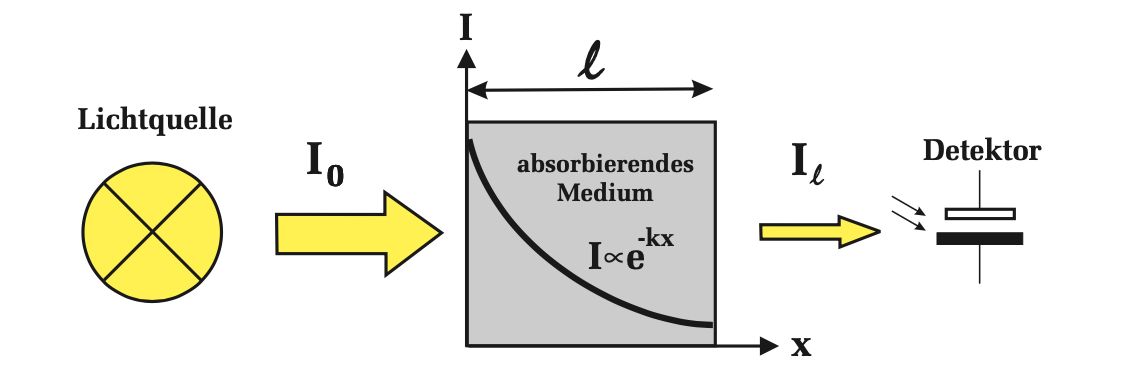
\includegraphics[width=0.7\textwidth]{img/principle.png}
    \caption{Schema des Labertschen Absorptionsgesetzes.\cite{PAPskript}}
    \caption*{Einfallendes Licht der Intensität $I_0$ wird beim Durchqueren einer absorbierenden Substanz der Dicke $l$ auf die Intensität $I$ abgeschwächt.}
    \label{fig:absorption}
\end{figure}

Mit den größen $\epsilon$ und $k'$ lässt sich das Absorptionsgesetz in der Form:
\begin{equation}
    I = I_0 \, 10^{-k' l} = I_0 \, 10^{-\epsilon c l}\label{eq:beer}\\
    = \log_{10}(I) =-\epsilon c l'
\end{equation}

mit $log_{10}$ auf beiden Seiten
\begin{equation}
    \log_{10}(I) = -\epsilon c l + \log_{10}(I_0)\label{Absorption}
\end{equation}

$\epsilon$ berechnet sich somit aus der Steigung der logarithmierten Intensität gegen die Konzentration $c$ bei einer festen Küvettenlänge $l$.



\subsection{Bestimmung des molaren Extinktionskoeffizienten}

Es werden in diesem Versuch 2 Messmethoden verwendet unm den molaren Extinktionskoeffizienten $\epsilon$ zu bestimmen. Zum einen wird die Absorption bei gleichbleibender Konzentratoin $c$ bei einer festen Wellenlänge gemessen. Die Steigung der logarithmierten Intensität gegen die länge liefert den Wert von $k'$. 
Mit Gleichung \ref{eq:Beersches Gesetz} kann dann $\epsilon$ berechnet werden.

Zum anderen wird die Absorption bei einer festen Wellenlänge für verschiedene Konzentrationen $c$ gemessen. Die Steigung der logarithmierten Intensität gegen die Konzentration liefert den Wert von $\epsilon$. 

\subsection{Dunkelmessung}
Die Dunkelmessung dient der Bestimmung der Hintergrundintensität, die durch das Messgerät selbst oder durch Umgebungslicht verursacht wird. Diese Hintergrundintensität wird von den gemessenen Intensitätswerten subtrahiert, um die tatsächliche Absorption der Probe zu erhalten.

\subsection{Literaturwerte}

Im Paper \cite{chebotarev2017} wird der molare Extinktionskoeffizient von Brillantblau FCF bei einer Wellenlänge von \SI{625}{\nano\meter} mit $\epsilon = \SI{0.97e5}{\liter\per\mole\per\centi\meter}$ angegeben \cite{chebotarev2017}. Dieser Wert dient als Referenz für die experimentell bestimmten Werte in diesem Versuch.




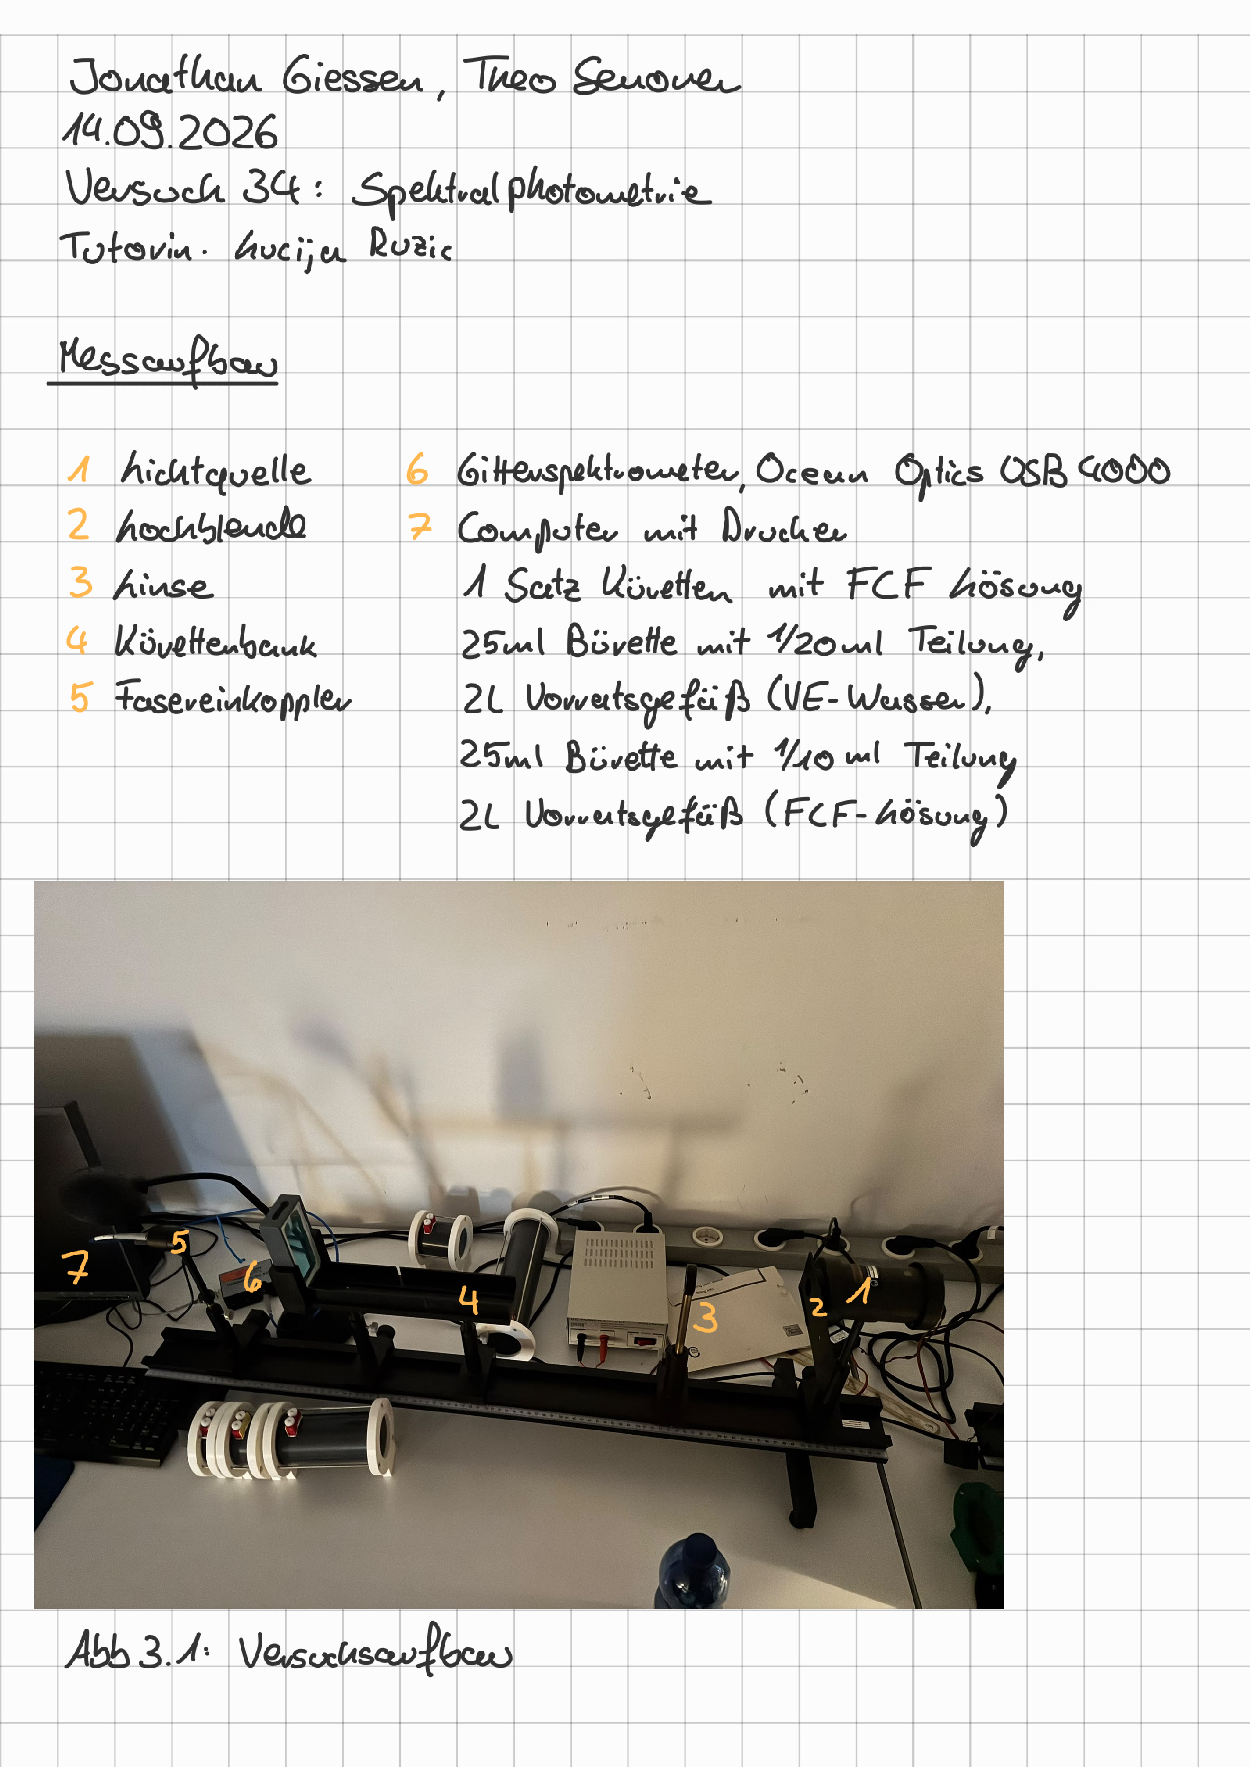
\includepdf[
    pages=-,
    width=\textwidth,
    height=0.95\textheight,
    keepaspectratio,
    pagecommand={\thispagestyle{scrheadings}},
    pagecommand*={\thispagestyle{scrheadings}\section{Messprotokoll}\subsection{Versuchsaufbau und Aufgaben}}
]{../Messprotokoll 34.pdf}

\pdfabbildung{Versuchsaufbau}{}
\pdfabbildung{Absorptionsmessung}{fig:absorptionsmessung}
\pdfabbildung{Bestimmung der Wellenlänge mit maximaler Absorption}{fig:pdf-3}
\pdfabbildung{Intensitätsspektrum}{fig:pdf-4}
\pdfabbildung{Halblogarithmischer Plot (Aufgabe 2,3)}{fig:pdf-5}
\pdftabelle{Intensität mit unterschiedlicher Längen}{tbl:pdf-1}
\pdftabelle{Intensität mit unterschiedlicher Konzentration}{tbl:pdf-2}

\subsection{Durchführung}

\paragraph{Aufgabe 1:}
Es wird eine Dunkelmessung durchgeführt, sowie einer Messung ohne Küvette, um die Intensität des Lichts zu bestimmen. Anschließend wird die Intensität des Lichts durch eine Küvette mit einer Lösung gemessen. Die gemessene Intensität wird von der Intensität des Lichts ohne Küvette subtrahiert, um die Absorptionswellenlänge der FCF-Lösung zu bestimmen. Die gemessene Wellenlänge beträgt $\lambda = \SI{629}{\nano\meter}$.

\paragraph{Aufgabe 2:}
Nun wird die Intensität des Lichts bei einer festen Wellenlänge von $\lambda = \SI{629}{\nano\meter}$ für verschiedene Küvettenlängen $l$ der FCF-Lösung gemessen. Dafür wird zuerst eine Dunkelmessung durchgeführt und danach die Intensitäten für die Wellenlänge $\lambda = \SI{629}{\nano\meter}$ bei den verschiedenen Küvettenlängen $l$ gemessen. Die Intensitätswerte werden logarithmiert und gegen die Küvettenlänge aufgetragen, um den dekadischen Absorptionskoeffizienten $k'$ zu bestimmen.

\paragraph{Aufgabe 3:}
Nun wird die Intensität des Lichts bei einer festen Wellenlänge von $\lambda = \SI{629}{\nano\meter}$ für verschiedene Konzentrationen $c$ der FCF-Lösung gemessen. Dafür wird zuerst eine Dunkelmessung durchgeführt und danach die Intensitäten für die Wellenlänge $\lambda = \SI{629}{\nano\meter}$ bei den verschiedenen Konzentrationen $c$ gemessen. Die Intensitätswerte werden logarithmiert und gegen die Konzentration aufgetragen, um den molaren Extinktionskoeffizienten $\epsilon$ zu bestimmen. 

Jeweils werden immer 5 Messungen pro Länge bzw. Konzentration durchgeführt, um den Mittelwert und die Standardabweichung zu bestimmen. Die Messwerte sind in den Tabellen \ref{tbl:pdf-1} und \ref{tbl:pdf-2} zusammengefasst.


\section{Auswertung}

\subsection{Berechnung der Steigung mithilfe des halblogarithmischen Plots}
Da die lange Küvette aufgrund des unterschiedlichen Brechungsindex der Lösung und der Luft wie eine Sammellinse wirkt, wird die Intensität des Lichts bei der langen Küvette verstärkt. Um die Intensitäten vergleichen zu können, wird der Durchmesser des Lichtkegels gemessen und mit dem Durchmesser des Lichtkegels ohne Küvette verglichen. Die Intensität kann dadurch mit dieser Korrekturformel korrigiert werden:
\begin{equation}
    I_\text{corr} = I \cdot \left(\frac{d_\text{mit Küvette}}{d_\text{ohne Küvette}}\right)^2\label{eq:Korrekturformel}
\end{equation}

Die Fehlerformel der Korrekturformel lautet:
\begin{equation}
    \Delta I_\text{corr} = I_\text{corr} \sqrt{\left(\frac{\Delta I}{I}\right)^2 + 4\left(\frac{\Delta d_\text{mit Küvette}}{d_\text{mit Küvette}}\right)^2 + 4\left(\frac{\Delta d_\text{ohne Küvette}}{d_\text{ohne Küvette}}\right)^2}
\end{equation}

Mit den folgenden Messwerten und Fehlern:
\begin{table}[H]
    \centering
    \caption{Messwerte und Fehler}
    \begin{tabular}{lc}
        \toprule
        Messsung & Wert\\
        \midrule
        Durchmesser 12mm: & $d_\text{12mm} = \num{7.0(6)}\,\si{\centi\meter}$\\
        Durchmesser 24mm: & $d_\text{24mm} = \num{5.4(6)}\,\si{\centi\meter}$\\
        Durchmesser ohne Küvette: & $d_0 = \num{9.0(6)}\,\si{\centi\meter}$\\
        Intensität 12mm: & $I_\text{12mm} = \num{2836(5)}$ cts\\
        Intensität 24mm: & $I_\text{24mm} = \num{241.0(2.9)}$ cts\\
        \bottomrule
    \end{tabular}
\end{table}

ergeben sich mit der Korrekturformel \ref{eq:Korrekturformel} die folgenden korrigierten Intensitäten:
\begin{align}
    I_\text{12mm,corr} &= \num{1720(370)}\\
    I_\text{24mm,corr} &= \num{87(23)}
\end{align}


Die korrigierten Intensitäten (Aus Tabelle \ref{tbl:pdf-1} und \ref{eq:Korrekturformel} berechnet) betragen nun: 

\begin{table}[H]
    \centering
    \caption{Korrigierte Intensitäten}
    \begin{tabular}{lc}
        \toprule
        Küvettenlänge $l$ & Korrigierte Intensität $I_\text{corr}$\\
        \midrule
        \SI{1.5}{\centi\meter} & \num{41200(700)}\\
        \SI{3}{\centi\meter} & \num{26660(170)}\\
        \SI{6}{\centi\meter} & \num{12952(4)}\\
        \SI{12}{\centi\meter} & \num{1720(370)}\\
        \SI{24}{\centi\meter} & \num{87(23)}\\
        \bottomrule
    \end{tabular}
\end{table}

Nun kann halblogarithmisch die Intensität gegen die Küvettenlänge aufgetragen werden, um die Steigung zu bestimmen. Die Steigung entspricht dem dekadischen Absorptionskoeffizienten $k'$.

\begin{figure}[H]
    \centering
    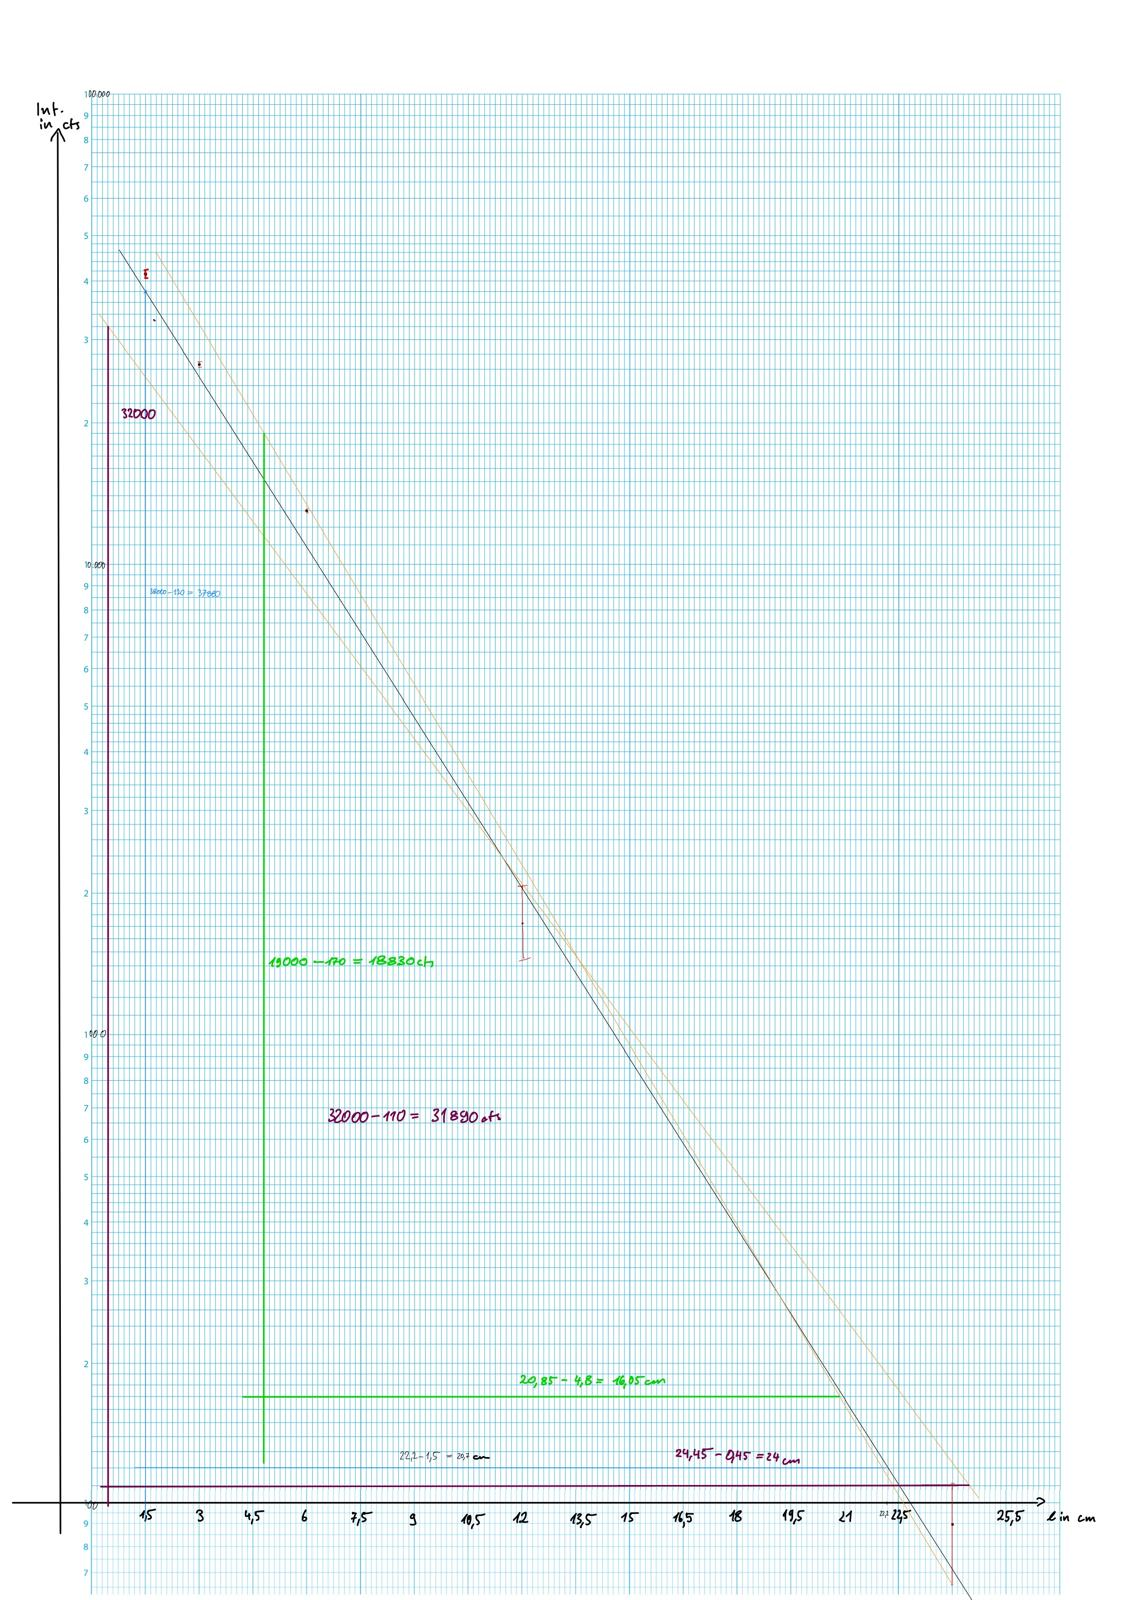
\includegraphics[width=0.8\textwidth]{img/A2.jpg}
    \caption{Intensitäten auf Halblogarithmischer Skala gegen die Küvettenlänge aufgetragen.}
    \label{fig:A2}
\end{figure}

Die Steigung der Geraden in Abbildung \ref{fig:A2} berechnen sich durch:
\begin{equation}
    k' = \frac{\log_{10}(I_1) - \log_{10}(I_2)}{l_2 - l_1}\label{Steigungformel}
\end{equation}

Aus den abgelesenen Steigungsdreiecken ergibt sich:
\begin{table}[H]
    \centering
    \caption{Steigung der Geraden}
    \begin{tabular}{lcccc}
        \toprule
        Art & $I_2$ [cts] & $I_1$ [cts] & $\Delta l_1$ [cm] & Ergebnis nach Gl. \ref{Steigungformel} [cts/\si{\centi\meter}]\\
        \midrule
        lower error & 32000 & 110 & 24 & $k' = 0.103$\\
        Mittelgerade & 38000 & 120 & 20.7 & $k' = 0.121$\\
        upper error & 18830 & 170& 16.05 & $k' = 0.127$\\
        \bottomrule
    \end{tabular}
\end{table}

Somit ergibt sich für $k'$ mit der Wert:
\begin{equation}
    k' =(\num{0.121(18)})\si{\per\centi\meter}
\end{equation}


Die verwendeten Küvetten besitzen eine Konzentration von $c = \SI{0.000001}{\mole\per\liter}$.
Aus dem lambertschen Absorptionsgesetz und dem Beerschen Gesetz (Gleichung \ref{eq:Beersches Gesetz}) ergibt sich für den molaren Extinktionskoeffizienten $\epsilon$:
\begin{equation}
    \epsilon = \frac{k'}{c} = \frac{(\num{0.121(18)})\si{\per\centi\meter}}{\num{0.000001}\si{\mole\per\liter}} = \num{1.21(18)e5e}\si{\liter\per\mole\per\centi\meter}
\end{equation}



\medspace
\begin{resultbox}[Ergebnis der Längenmessung]
    Der molare Extinktionskoeffizient $\epsilon$ mithilfe der Längenmessung beträgt:
    \begin{equation*}
        \epsilon = \num{1.21(18)e5}\si{\liter\per\mole\per\centi\meter}
    \end{equation*}

\end{resultbox}

\subsection{Berechnung der Steigung mithilfe der Konzentrationsmessung}

Die Konzentration wurde mithilfe von Hinzugeben von verdünnter Lösung in die Küvette verändert. Die Konzentration der verdünnten Lösung wurde mit der Pipette bestimmt. 

Um die Konzentration der Lösung in der Küvette zu bestimmen, wird die Formel:
\begin{equation}
    c_k = c_0 \frac{\sum_{i=1}^{k}V_i}{V_0 + \sum_{i=1}^{k}V_i} \text{für } k \in [0{,} 5]\footnotemark
\end{equation}
\footnotetext{$\sum_{i=1}^{0} V_i \coloneq 0$}
verwendet.
Die Fehlerformel für die Konzentration, wenn $c$ ohne fehler ist:
\begin{align}
\Delta c_k &= \sqrt{ \left( \frac{\partial c_k}{\partial V_0} \Delta V_0 \right)^2 + \sum_{i=1}^k \left( \frac{\partial c_k}{\partial V_i} \Delta V_i \right)^2 }\\
 &=\footnotemark \frac{c_0}{\left(V_0 + \sum_{i=1}^k V_i\right)^2} \sqrt{ \left( \sum_{i=1}^k V_i \right)^2 (\Delta V_0)^2 + V_0^2 \sum_{i=1}^k (\Delta V_i)^2 }\label{Fehlerformel C}
\end{align}
\footnotetext{Danke an Daddy Gemini, keine Ahnung wie ich das Ableite}

Mit den folgenden Werten:
\begin{table}[H]
    \caption{Parameter für die Konzentrationsberechnung}
    \centering
    \begin{tabular}{rl}
        \toprule
        Variable & Wert\\
        \midrule
        $c_0 = $ & $(\num{5e-6})\,\si{\mole\per\liter}$\\
        $V_0 = $ & $(\num{21.0(3)})\,\si{\milli\liter}$\\
        $V_1 = $ & $(\num{1.4(3)})\,\si{\milli\liter}$\\
        $V_2 = $ & $(\num{1.6(3)})\,\si{\milli\liter}$\\
        $V_3 = $ & $(\num{4.0(3)})\,\si{\milli\liter}$\\
        $V_4 = $ & $(\num{14.0(3)})\,\si{\milli\liter}$\\
        \bottomrule
    \end{tabular}

\end{table}

ergeben sich die folgenden Konzentrationen und Intensitäten:

\begin{table}[H]
    \centering
    \caption{Messwerte der Konzentrationsmessung}
    \begin{tabular}{lcc}
        \toprule
        $i$ & Konzentration $c$ [\si{\mole\per\liter}] & Intensität $I$ [cts]\\
        \midrule
        0 & $c_0 = $ 0 & \num{51568(26)}\\
        1 & $c_1 = $ \num{0.31(6)e-6} & \num{47280(90)}\\
        2 & $c_2 = $ \num{0.63(8)e-6} & \num{39930(60)}\\
        3 & $c_3 = $ \num{1.25(7)e-6} & \num{34180(50)}\\
        4 & $c_4 = $ \num{2.50(4)e-6} & \num{18592(28)}\\
        \bottomrule
    \end{tabular}
\end{table}

Nun werden die logarithmierten Intensitäten gegen die Konzentration aufgetragen, um die Steigung zu bestimmen:

\begin{figure}[H]
    \centering
    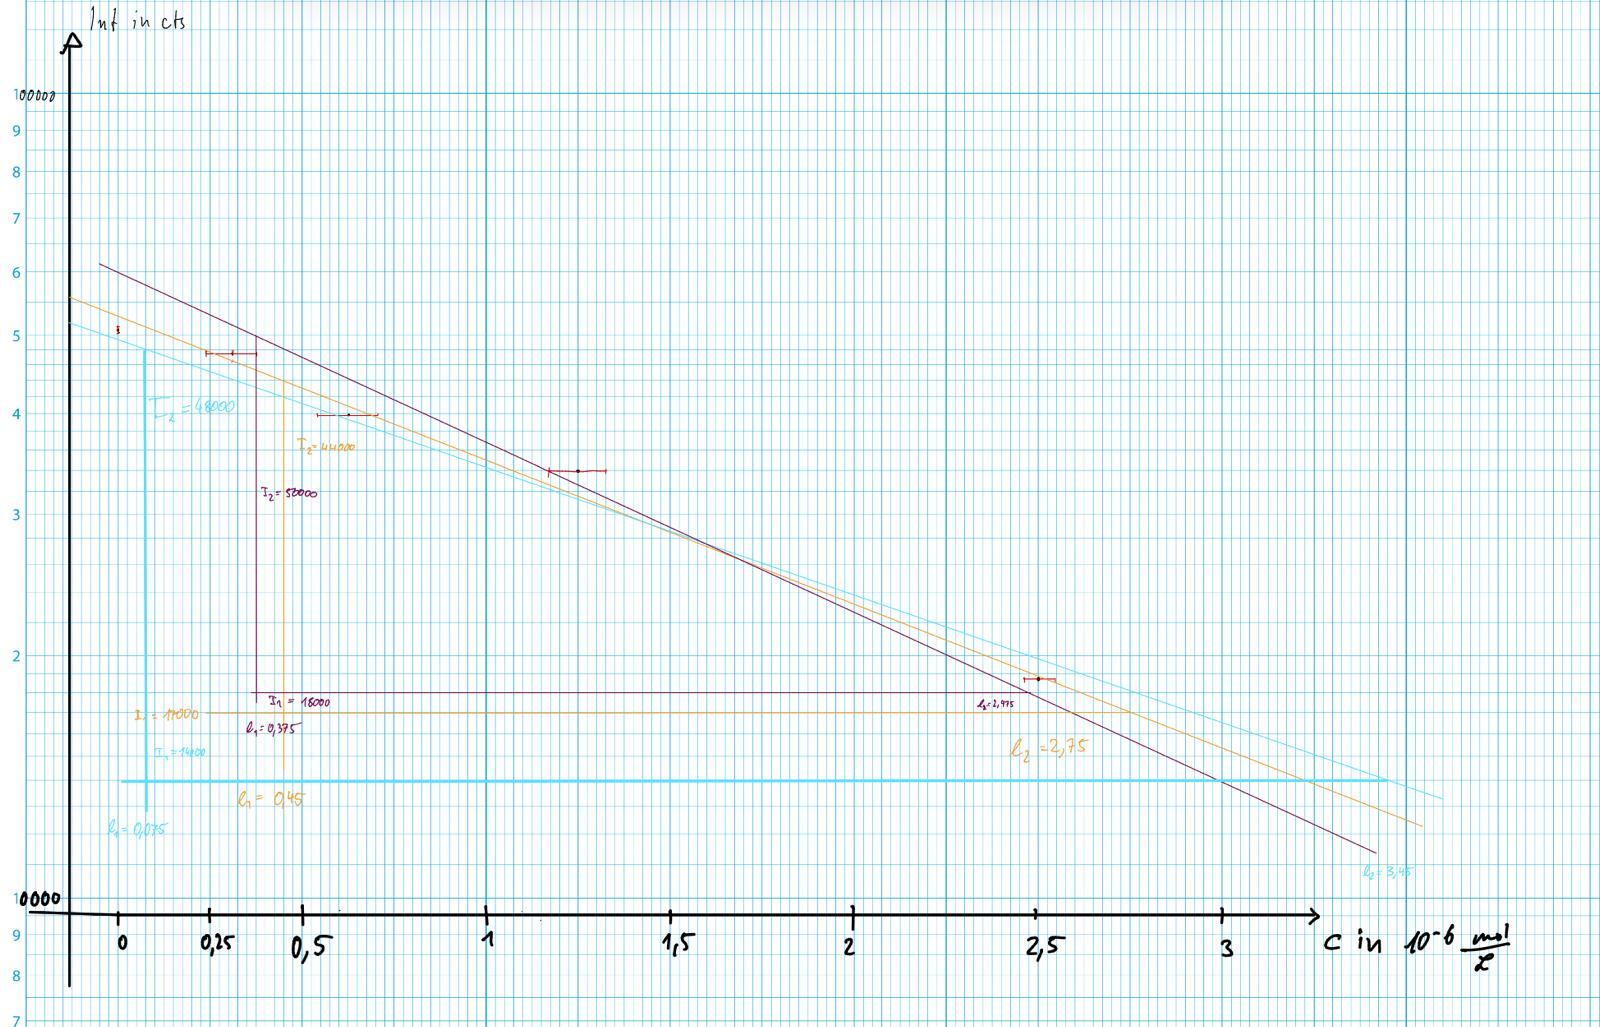
\includegraphics[width=\textwidth]{img/A3.jpg}
    \caption{Intensitäten auf Halblogarithmischer Skala gegen die Konzentration aufgetragen.}
    \label{fig:A3}
\end{figure}

Der Molare Extinktionskoeffizient $\epsilon$ berechnet sich aus der Steigung der Geraden in Abbildung \ref{fig:A3} und Gleichung \ref{Absorption}:

\begin{equation}
    \epsilon = \frac{\log_{10}(I_2) - \log_{10}(I_1)}{(c_2 - c_1) \cdot l}\label{Steigungformel_Konzentration}
\end{equation}

\begin{table}[H]
    \centering
    \caption{Werte für die Steigungsberechnung (mit $l = \SI{1.5}{\centi\meter}$)}
    \begin{tabular}{lcccc}
        \toprule
        Art & $I_2$ [cts] & $I_1$ [cts] & $\Delta c$ [\si{\mole\per\liter}] & Ergebnis nach Gl. \ref{Steigungformel_Konzentration} [\si{\liter\per\mole\per\centi\meter}]\\
        \midrule
        lower error & 48000 & 14000 & \num{3.375e-6} & $\epsilon = \num{1.06e5}$\\
        Mittelgerade & 44000 & 17000 & \num{2.3e-6} & $\epsilon = \num{1.20e5}$\\
        upper error & 50000 & 18000 & \num{2.1e-6} & $\epsilon = \num{1.41e5}$\\
        \bottomrule
    \end{tabular}
\end{table}


\begin{resultbox}[Ergebnis der Konzentrationsmessung]
    Der molare Extinktionskoeffizient $\epsilon$ mithilfe der Konzentrationsmessung beträgt:
    \begin{equation*}
        \epsilon = \num{1.20(21)e5}\si{\liter\per\mole\per\centi\meter}
    \end{equation*}
\end{resultbox}


\subsection{Abweichung der Messwerte}

\begin{table}[H]
    \centering
    \caption{Berechnete Werte und Literaturwert}
    \begin{tabular}{lc}
        \toprule
        Methode & $\epsilon$ [\si{\liter\per\mole\per\centi\meter}]\\
        \midrule
        Längenmessung & \num{1.21(18)e5}\\  
        Konzentrationsmessung & \num{1.20(21)e5}\\
        Literaturwert & \num{0.97e5}\\
        \bottomrule
    \end{tabular}
\end{table}

Die Sigma-Abweichung der Messwerte zum Literaturwert beträgt:
\begin{align}
    \sigma_\text{len} &= \frac{|\epsilon_\text{len} - \epsilon_\text{Lit}|}{\Delta \epsilon_\text{len}} = \frac{|\num{1.21e5} - \num{0.97e5}|}{\num{0.18e5}} = 1.33 &\Rightarrow 1.33\sigma\\
    \sigma_\text{conc} &= \frac{|\epsilon_\text{conc} - \epsilon_\text{Lit}|}{\Delta \epsilon_\text{conc}} = \frac{|\num{1.20e5} - \num{0.97e5}|}{\num{0.21e5}} = 1.10 &\Rightarrow 1.10\sigma
\end{align}

Die Sigma-Abweichung der beiden Messwerte beträgt:
\begin{align}
    \sigma_\text{len-conc} &= \frac{|\epsilon_\text{len} - \epsilon_\text{conc}|}{\sqrt{\Delta \epsilon_\text{len}^2 + \Delta \epsilon_\text{conc}^2}} = \frac{|\num{1.21e5} - \num{1.20e5}|}{\sqrt{\left(\num{0.18e5}\right)^2 + \left(\num{0.21e5}\right)^2}} = 0.03 &\Rightarrow 0.03\sigma
\end{align}

\begin{resultbox}[Abweichung der Messwerte]
    Die Abweichungen der Messwerte betragen:
    \begin{align*}
        \sigma_\text{len} &= 1.33\sigma\\
        \sigma_\text{conc} &= 1.10\sigma\\
        \sigma_\text{len-conc} &= 0.03\sigma
    \end{align*}
\end{resultbox}

\section{Diskussion}

Die Abweichung der beiden Messmethoden von nur $0.03\sigma$ beweist die Konstenz der Messmethodik. Es ist zu erkennen, dass die Abweichung der Messwerte zum Literaturwert bei beiden Messmethoden größer als $1\sigma$ beträgt. Dies zeigt, dass die Messmethoden zwar konsistent sind, aber systematische Fehler in der Versuchsdurchführung oder in der Kalibrierung des Messgeräts vorliegen könnten. Mögliche Ursachen für diese Abweichungen könnten ungenaue Pipettierungen, Schwankungen in der Lichtquelle oder unzureichende Berücksichtigung von Streulicht sein.

Dass der experimentell ermittelte Extinktionskoeffizient deutlich über dem Literaturwert liegt, lässt sich vor allem auf die gewählte Messwellenlänge zurückführen. Die Messung erfolgte im experimentell bestimmten Absorptionsmaximum bei $\lambda = 629\text{ nm}$, während der zitierte Literaturwert für $\lambda = 625\text{ nm}$ angegeben ist. Da der molare Extinktionskoeffizient stark wellenlängenabhängig ist und die Absorption an der Peak-Wellenlänge am stärksten ausfällt, resultiert hieraus physikalisch direkt ein größerer Wert für $\epsilon$. Darüber hinaus können Streuverluste durch winzige Kratzer oder Verunreinigungen (wie Fingerabdrücke) auf den Küvettenwänden die durchtretende Lichtintensität zusätzlich abgeschwächt haben. Dies wird photometrisch als höhere Absorption interpretiert und hebt den Wert von $\epsilon$ weiter künstlich an.

\medskip
Ein weiterer wichtiger Hinweis zur systematischen Fehlerbetrachtung findet sich im Datenblatt des FCF-Farbstoffs. Dort sind unter anderem die Angaben:
\begin{quote}
    \emph{Loss on Drying: $\le 13\%$}\\
    \emph{In H2O insoluble matter: $\le 1\%$}
\end{quote}

Da das Pulver stark hygroskopisch ist, bedeutet dies, dass bis zu $14\%$ der beim Herstellen der Lösung gewogenen Masse kein reiner Farbstoff, sondern Wasser und andere Verunreinigungen sind. Somit ist die tatsächliche Konzentration der verwendeten Stammlösung niedriger als die nominell angegebenen $5 \cdot 10^{-6} \, \frac{\text{mol}}{\text{L}}$. Da die Konzentration bei der Berechnung des Extinktionskoeffizienten im Nenner steht, würde dieser systematische Fehler rechnerisch jedoch zu einem noch größeren theoretischen Wert für $\epsilon$ führen. Dieser Umstand der mangelnden Reinheit kann die Diskrepanz zum Literaturwert somit nicht erklären, sondern verdeutlicht, dass die Effekte der Wellenlängenabweichung und der Streuverluste dominant sein müssen.



\section{Fazit}
Zum Ende lässt sich sagen, dass die Spektralphotometrie eine effektive Methode zur Bestimmung des molaren Extinktionskoeffizienten von Brillantblau FCF ist. Beide Messmethoden, die Längenmessung und die Konzentrationsmessung, lieferten konsistente Ergebnisse, die jedoch leicht vom Literaturwert abwichen. Die Abweichungen können auf systematische Fehler und Unsicherheiten in der Probenvorbereitung zurückgeführt werden. Zukünftige Experimente könnten durch präzisere Pipettierung, sorgfältigere Kontrolle der Probenkonzentration und Berücksichtigung von Streulicht verbessert werden. Der Versuch war sehr interessant und lehrreich, da er sowohl die theoretischen Grundlagen der Fotometrie als auch praktische Fähigkeiten in der experimentellen Physik vermittelte. Die Messmethode war einfach durchzuführen. 




\clearpage

\listoffigures


\listoftables

\begin{thebibliography}{5}
    \bibitem{PAPskript} Dr. J.Wagner, \emph{Physikalisches Anfängerpraktikum}, Stand 11/2024
    \bibitem{ilberg1988physikalisches} W. Ilberg, M. Krötzsch, \emph{Physikalisches Praktikum für Anfänger}, BSB B. G. Teubner Verlagsgesellschaft, Leipzig (1985).
    \bibitem{chebotarev2017} A. Chebotarev, K. Bevziuk, D. Snigur und Y. Bazel, ``The brilliant blue FCF ion-molecular forms in solutions according to the spectrophotometry data'', \emph{Russian Journal of Physical Chemistry A}, 91, 1907--1912 (2017). DOI: \href{https://doi.org/10.1134/S0036024417100089}{10.1134/S0036024417100089}.
    
\end{thebibliography}

\appendix
\section{Anhang - Code}

    
    \begin{tcolorbox}[breakable, size=fbox, boxrule=1pt, pad at break*=1mm,colback=cellbackground, colframe=cellborder]
\prompt{In}{incolor}{2}{\boxspacing}
\begin{Verbatim}[commandchars=\\\{\}]
\PY{k+kn}{import}\PY{+w}{ }\PY{n+nn}{numpy}\PY{+w}{ }\PY{k}{as}\PY{+w}{ }\PY{n+nn}{np}
\end{Verbatim}
\end{tcolorbox}

    \begin{tcolorbox}[breakable, size=fbox, boxrule=1pt, pad at break*=1mm,colback=cellbackground, colframe=cellborder]
\prompt{In}{incolor}{ }{\boxspacing}
\begin{Verbatim}[commandchars=\\\{\}]
\PY{n}{c0} \PY{o}{=} \PY{n}{np}\PY{o}{.}\PY{n}{array}\PY{p}{(}\PY{p}{[}\PY{l+m+mi}{51545}\PY{p}{,} \PY{l+m+mi}{51483}\PY{p}{,} \PY{l+m+mi}{51625}\PY{p}{,} \PY{l+m+mi}{51615}\PY{p}{,} \PY{l+m+mi}{51549}\PY{p}{]}\PY{p}{)}
\PY{n}{c1} \PY{o}{=} \PY{n}{np}\PY{o}{.}\PY{n}{array}\PY{p}{(}\PY{p}{[}\PY{l+m+mi}{47577}\PY{p}{,} \PY{l+m+mi}{47315}\PY{p}{,} \PY{l+m+mi}{47219}\PY{p}{,} \PY{l+m+mi}{47096}\PY{p}{,} \PY{l+m+mi}{47206}\PY{p}{]}\PY{p}{)}
\PY{n}{c2} \PY{o}{=} \PY{n}{np}\PY{o}{.}\PY{n}{array}\PY{p}{(}\PY{p}{[}\PY{l+m+mi}{40052}\PY{p}{,} \PY{l+m+mi}{40003}\PY{p}{,} \PY{l+m+mi}{39741}\PY{p}{,} \PY{l+m+mi}{39913}\PY{p}{,} \PY{l+m+mi}{39952}\PY{p}{]}\PY{p}{)}
\PY{n}{c3} \PY{o}{=} \PY{n}{np}\PY{o}{.}\PY{n}{array}\PY{p}{(}\PY{p}{[}\PY{l+m+mi}{34170}\PY{p}{,} \PY{l+m+mi}{34188}\PY{p}{,} \PY{l+m+mi}{34145}\PY{p}{,} \PY{l+m+mi}{34061}\PY{p}{,} \PY{l+m+mi}{34315}\PY{p}{]}\PY{p}{)}
\PY{n}{c4} \PY{o}{=} \PY{n}{np}\PY{o}{.}\PY{n}{array}\PY{p}{(}\PY{p}{[}\PY{l+m+mi}{18601}\PY{p}{,} \PY{l+m+mi}{18644}\PY{p}{,} \PY{l+m+mi}{18496}\PY{p}{,} \PY{l+m+mi}{18573}\PY{p}{,} \PY{l+m+mi}{18646}\PY{p}{]}\PY{p}{)}

\PY{k}{def}\PY{+w}{ }\PY{n+nf}{calculate\PYZus{}mean}\PY{p}{(}\PY{n}{data}\PY{p}{)}\PY{p}{:}
    \PY{n}{s} \PY{o}{=} \PY{n}{np}\PY{o}{.}\PY{n}{std}\PY{p}{(}\PY{n}{data}\PY{p}{,} \PY{n}{ddof}\PY{o}{=}\PY{l+m+mi}{1}\PY{p}{)}\PY{o}{/}\PY{n}{np}\PY{o}{.}\PY{n}{sqrt}\PY{p}{(}\PY{n+nb}{len}\PY{p}{(}\PY{n}{data}\PY{p}{)}\PY{p}{)}
    \PY{n+nb}{print}\PY{p}{(}\PY{n}{np}\PY{o}{.}\PY{n}{mean}\PY{p}{(}\PY{n}{data}\PY{p}{)}\PY{p}{,} \PY{n}{s}\PY{p}{)}
    
\PY{n}{calculate\PYZus{}mean}\PY{p}{(}\PY{n}{c0}\PY{p}{)}
\PY{n}{calculate\PYZus{}mean}\PY{p}{(}\PY{n}{c1}\PY{p}{)}
\PY{n}{calculate\PYZus{}mean}\PY{p}{(}\PY{n}{c2}\PY{p}{)}
\PY{n}{calculate\PYZus{}mean}\PY{p}{(}\PY{n}{c3}\PY{p}{)}
\PY{n}{calculate\PYZus{}mean}\PY{p}{(}\PY{n}{c4}\PY{p}{)}
\end{Verbatim}
\end{tcolorbox}

    \begin{Verbatim}[commandchars=\\\{\}]
51563.4 25.949181104612915
47282.6 81.37972720524442
39932.2 53.23664151691013
34175.8 41.040711494807205
18592.0 27.63874092646045
    \end{Verbatim}

    concentration

    \begin{tcolorbox}[breakable, size=fbox, boxrule=1pt, pad at break*=1mm,colback=cellbackground, colframe=cellborder]
\prompt{In}{incolor}{ }{\boxspacing}
\begin{Verbatim}[commandchars=\\\{\}]
\PY{l+m+mi}{67}
\end{Verbatim}
\end{tcolorbox}




\end{document}